% Resultados

\chapter*{Resultados} \label{cap6}
\addcontentsline{toc}{chapter}{Resultados}

\begin{flushright}
\begin{minipage}{7.85cm}
    {\em Si buscas resultados distintos, no hagas siempre lo mismo.} \\ Albert
    Einstein
\end{minipage}
\end{flushright}

\vspace*{5mm}

\section*{Preparando el Escenario}

Para poder validar el trabajo realizado, hemos de simular lo ocurrido en el
caso guía y comparar los resultados con lo que realmente pasó. Para ello hemos
recopilado información de la inundación provocada por el paso del huracán
Katrina por Nueva Orleans en el año 2005.

Utilizando la información obtenida, creamos un escenario de simulación que
recrea la catástrofe que asoló la ciudad de Nueva Orleans. Como datos de
entrada utilizamos las roturas de los diques que contenían al río Mississippi
-nuestras Entradas de Agua-, la distribución de la población -los agentes
Peatón-, el terreno real y las calles reales de la ciudad.

\subsection*{Área de simulación}

El huracán Katrina afectó a una parte considerable del estado de Luisiana, pero
nosotros nos centraremos en la ciudad de Nueva Orleans. En concreto el área que
se inundó de la ciudad viene resaltada en la siguiente imagen.

\begin{figure}[H]
 \centering
 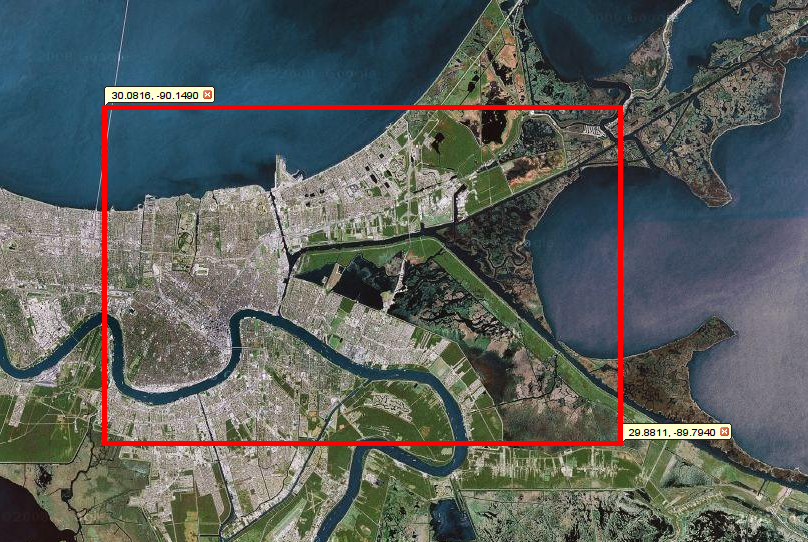
\includegraphics[height=120mm,angle=90]{figuras/cap6/NOarea1.png}
 \caption{Área de Simulación}
\end{figure}

Al producirse la inundación por el desbordamiento del río, entre el mismo río y
los canales que atraviesan la ciudad dividieron la inundación en tres grandes
zonas casi independientes. En la siguiente imagen se puede apreciar la división
de la inundación en las tres zonas afectadas.

\begin{figure}[H]
 \centering
 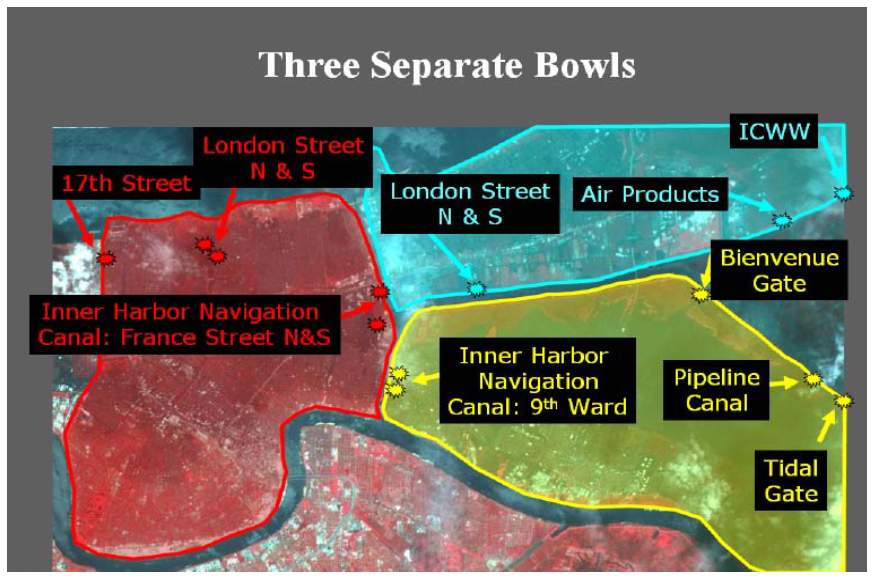
\includegraphics[width=100mm]{figuras/cap6/affected.png}
 \caption{División en zonas del área afectada}
\end{figure}

Al ser el mismo río el que separa las diferentes zonas, éstas pueden simularse
por separado. Para ahorrar recursos y reducir la carga computacional nos
planteamos la creación de tres escenarios de simulación separados. Las
siguientes imágenes muestran las áreas de cada uno de dichos escenarios.

\begin{figure}[H]
 \centering
 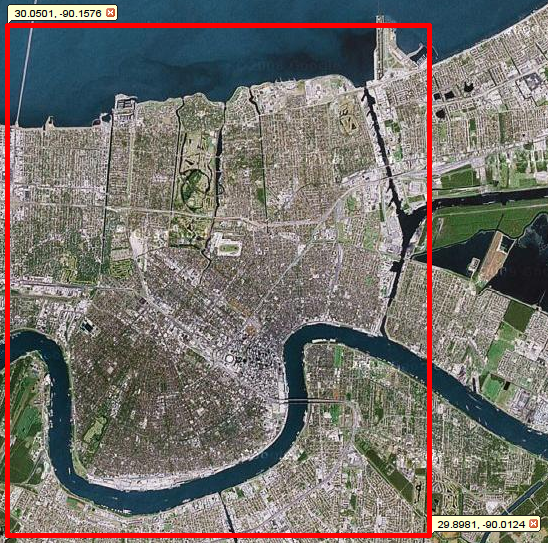
\includegraphics[width=120mm]{figuras/cap6/NOarea2.png}
 \caption{Zona 1 de simulación}
\end{figure}

\begin{figure}[H]
 \centering
 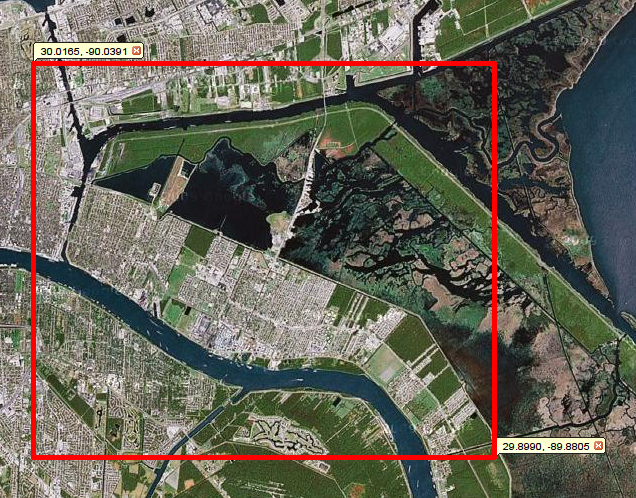
\includegraphics[width=135mm]{figuras/cap6/NOarea3.png}
 \caption{Zona 2 de simulación}
\end{figure}

\begin{figure}[H]
 \centering
 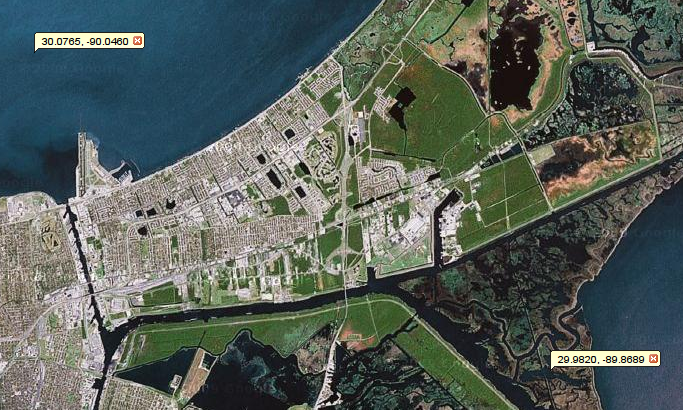
\includegraphics[width=135mm]{figuras/cap6/NOarea4.png}
 \caption{Zona 3 de simulación}
\end{figure}


\subsection*{Obteniendo Alturas}

Para poder simular la inundación uno de los datos que tenemos que obtener son
las alturas, para una zona tan grande como Nueva Orleans hacen falta millones
de datos de altura, sin embargo para nuestra simulación nos hemos limitado a la
parte de nueva orleans que resultó mas afectada y con una precision de 50
metros por casilla.

\subsection*{Localización de las roturas de los diques}

De este mapa podemos ver las localizaciones donde los diques se rompieron.

\begin{figure}[H]
 \centering
 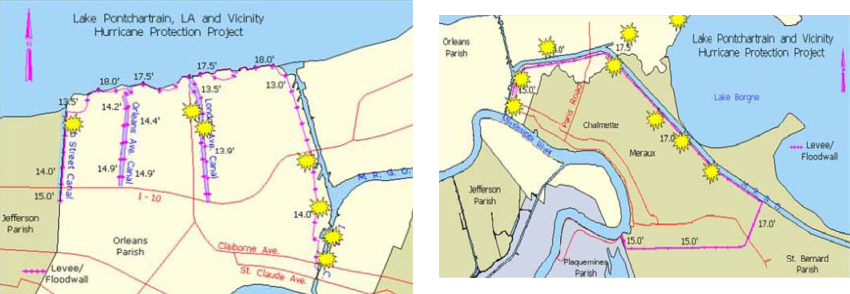
\includegraphics[width=135mm]{figuras/cap6/dikes.png}
 \caption{Mapa con las localizaciones de las roturas de los diques}
\end{figure}

A continuación mostramos la información con la que hemos realizado la
simulación de donde se encontraban los diques.

% \begin{figure}[H]
%  \centering
%  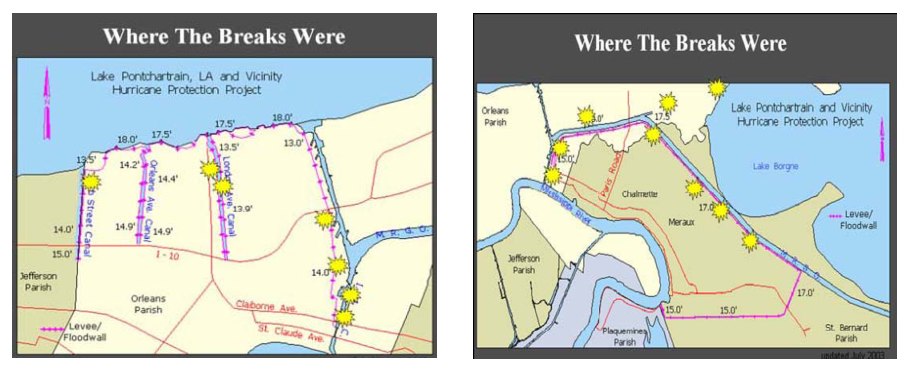
\includegraphics[width=30mm]{figuras/cap6/Roturas de Diques.png}
%  % NOarea1.png: 1066x626 pixel, 96dpi, 28.20x16.56 cm, bb=0 0 799 469
% \caption{Mapa con las localizaciones de las roturas de los diques}
% \end{figure}

\begin{figure}[H]
 \centering
 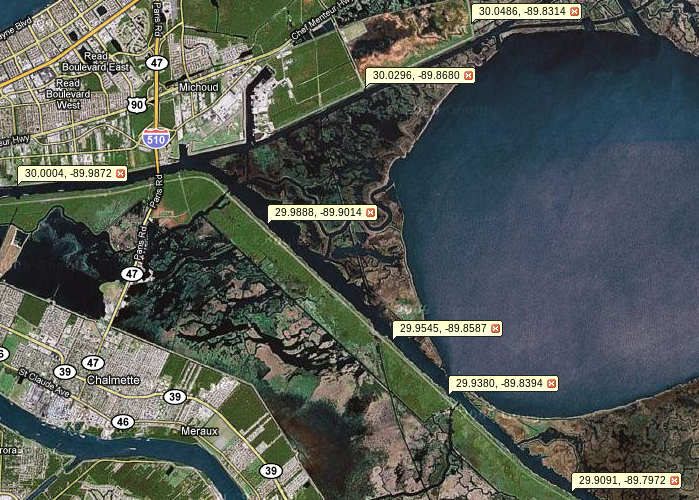
\includegraphics[width=135mm]{figuras/cap6/dikes1.png}
 \caption{Detalle de las roturas de los diques 1}
\end{figure}


\begin{figure}[H]
 \centering
 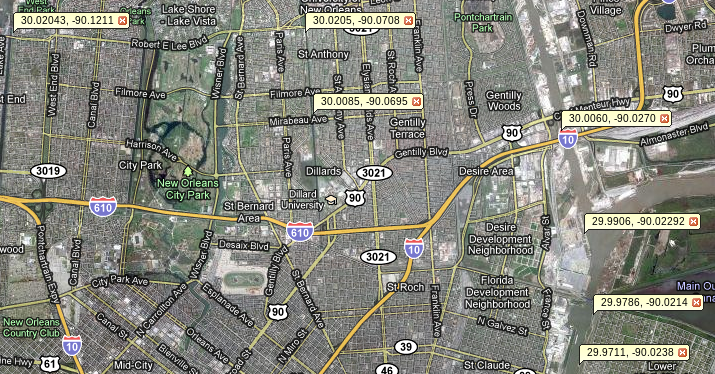
\includegraphics[width=140mm]{figuras/cap6/dikes2.png}
 \caption{Detalle de las roturas de los diques 2}
\end{figure}

\subsection*{Rutas de evacuación y refugios}

Refugios oficiales no hubo en la inundación, lo que se hizo fue una evacuación
completa de la ciudad, para ello, hemos marcado como objetivo tres posibles
rutas de escape para los ciudadanos.

También consideramos que los edificios de los cuales podemos obtener
información a través de OSM pudieron ser refugios de emergencia donde
temporalmente pudieron refugiarse algunos ciudadanos.

\begin{figure}[H]
 \centering
 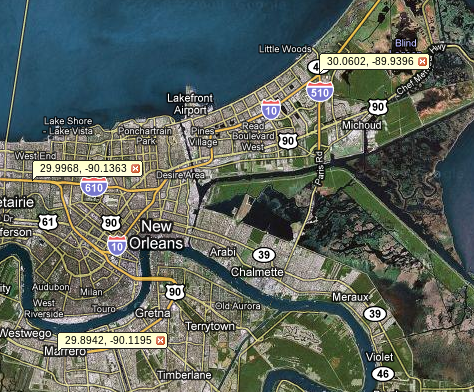
\includegraphics[width=100mm]{figuras/cap6/evacuation.png}
 \caption{Rutas de evacuación}
\end{figure}

\section*{Resultados}
%echamos a correr el simulador y comentamos la jugada
\subsection*{Visualización de Resultados}
%Ventanitas del simulador o capturas de google earth
\section*{Simulación frente Realidad}
%Es cuestion de preparar un escenario de nueva orleans y comparar con la
%bibliografia

%%% Local Variables:
%%% mode: latex
%%% TeX-master: "../dissim"
%%% End: